\documentclass{standalone}

\usepackage{tikz}
\usepackage{pgfplots}

\usetikzlibrary{arrows.meta}
\usetikzlibrary{positioning}

\begin{document}
\begin{tikzpicture}

    % Define the nodes for the PDFs
    \node[anchor=south west,inner sep=0] (pdf1) at (0,0) {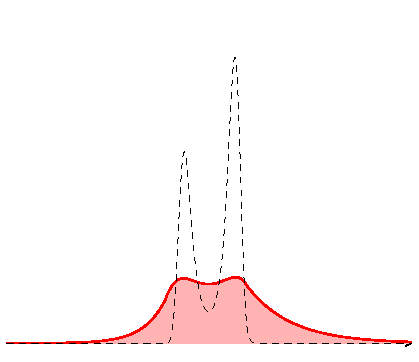
\includegraphics[width=0.25\textwidth]{pdf_i.pdf}};
    \node[anchor=south west,inner sep=0] (pdf2) at (4,0) {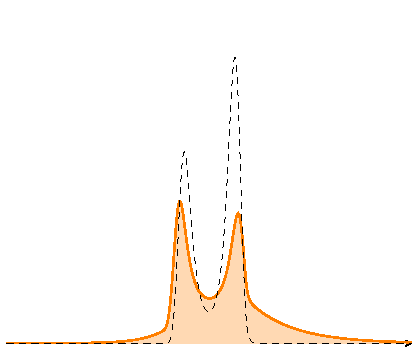
\includegraphics[width=0.25\textwidth]{pdf_t.pdf}};
    % \node[anchor=south west,inner sep=0] (pdf3) at (8,0) {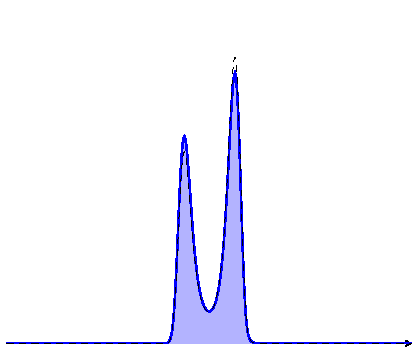
\includegraphics[width=0.25\textwidth]{pdf_m.pdf}};
    \node[anchor=south west,inner sep=0] (pdf4) at (8,0) {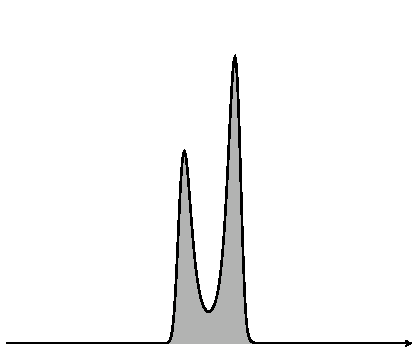
\includegraphics[width=0.25\textwidth]{pdf_s.pdf}};
    
    % Draw the arrows connecting the PDFs
    \draw[->, thick] ([yshift=-0.5cm]pdf1.east) -- ([yshift=-0.5cm]pdf2.west);
    % \draw[->, thick] ([yshift=-0.5cm]pdf2.east) -- ([yshift=-0.5cm]pdf3.west);
    % \draw[->, thick] ([yshift=-0.5cm]pdf3.east) -- ([yshift=-0.5cm]pdf4.west);
    \draw[->, thick] ([yshift=-0.5cm]pdf2.east) -- ([yshift=-0.5cm]pdf4.west);

\end{tikzpicture}
\end{document}